\documentclass{report}
\usepackage[T1]{fontenc}
\usepackage{lmodern}
\usepackage[utf8]{inputenc}

% Newline instead of indent for paragraph
\usepackage[parfill]{parskip}

% Bold \emph 
\renewcommand{\emph}[1]{\textbf{#1}}

% Description environment
\usepackage{enumitem}

% Math stuff like \DeclareMathOperator
\usepackage{amsmath}

% Algorithm descriptions
\usepackage[ruled,vlined]{algorithm2e}

% Plots such as FAR/FRR
\usepackage{pgfplots}
\pgfplotsset{compat=1.17}

% Links for TOC and refs
\usepackage{hyperref}

% References with name of item etc
\usepackage{cleveref}

% UML diagrams
\usepackage{tikz-uml}

\usepackage{todonotes}

\DeclareMathOperator{\hash}{hash}

\title{Lecture Notes: Security of IT-Systems}
\author{Jonas Otto}

\begin{document}

\maketitle

\listoftodos

\tableofcontents

\chapter{Fundamentals}
\section{Motivation and Introduction}
The number of catalogued vulnerabilities is rising rapidly over time, ever since
IT existed. Security is all over the headlines both in dedicated news agencies
and in mainstream media. Ransomware attacks are popular recently and have highly
visible and critical targets such as hospitals and large companies. Running a
networked computer system with 100\% security is neither feasible nor possible.
But strong security is still achievable, and defending most attackers is
possible.

\section{Terminology}
When talking about ``secure'' systems, what is usually desired is a
``dependability'', meaning a system that shows no unexpected or unacceptable
behavior. A dependable system should fulfill multiple goals, including
\begin{itemize}
    \item \emph{Availability}
    \item Reliability
    \item Safety
    \item \emph{Integrity}
    \item Maintainability
    \item \emph{(Confidentiality)}
\end{itemize}

The three major security goals are Confidentiality, Integrity and Availability
(\emph{CIA}). The main difference between dependability and security is that the
security is usually assessed from the viewpoint of a potential attack, while
dependability is considered in a more general context. Security can be seen as a
precondition of having a dependable system. A secure system is a system that can
achieve the three mentioned goals even facing an attacker.

\begin{description}[align=right,labelwidth=3cm]
    \item[Confidentiality] Protection of information against unauthorized access
    \item[Integrity] Protection against unauthorized change and destruction
    \item[Availability] Protection against rendering IT resources inaccessible
\end{description}

A \emph{threat} is defined by a potential error in the system, which could
enable an attacker to violate those objectives. A \emph{vulnerability} is a
concrete fault in the system that threaten one or more security objective. A
threat would be for example the possibility of a DDOS attack towards a web
service, a lack of resources to cope with the attack is a vulnerability. If an
attacker exploits the vulnerability, this is called an \emph{attack}.

The concepts of safety and security shall be differentiated.

When analyzing a system with regards to it security, two factors are considered:
The first is \emph{threat potential}, which estimates the likelihood of each
potential attack against the system. The second is the \emph{damage potential},
which asks what the impact to the system would be if an attack succeeds. Likely
high-impact attack scenarios can be mitigated by either reducing the impact of a
successful impact or by taking security measures reducing the likelihood of a
successful attack.

A few more useful definitions:
\begin{description}[align=right,labelwidth=3cm]
    \item[Identification] Assignment of an identifier
    \item[Authentication] Verification of an identity
    \item[Authorization] Assignment of permissions
    \item[Access Control] Protection of resources against unauthorized access
    \item[Privacy] Protecting personal information
\end{description}

\section{Attacks and Defenses}
\subsection{Attacks}
Attack can be categorized by many measures, like intention, approach or point of
attack.

Categories by intention can be:
\begin{description}
    \item[Denial of Service ]Making an IT system unabailable to users
    \item[Information Theft] Access to confidential information by unauthorized
          persons
    \item[Intrusion] Bypassing access control to gain access to a system
    \item[Tampering] Modification of stored or transmitted data
\end{description}

By approach:
\begin{itemize}
    \item Masquerading
    \item Eavesdropping
    \item Authorization Violation
    \item Loss/Modification
    \item Denial/Repudiation
    \item Forgery
    \item Sabotage
\end{itemize}

By point of attack:
\begin{itemize}
    \item Network
    \item Network services
    \item Operating system/Applications
    \item User
\end{itemize}

Another possible method of categorization is ``STRIDE'' categorization, which
stands for Spoofing, Tampering, Repudiation, Information disclosure, Denial of
Service and Elevation of privilege.

An attack often follows similar patterns. The first step is collecting
information of the system. This may expose a possible attack vector to the
attacker, which can then be used/tested. This is often repeated, as the first
attack is not necessarily successful. After a successful intrusion the next step
is often privilege escalation. This may allow the attacker to cover their
tracks, install back doors, etc. If the main goal of the attack is not reached
yet, this point may be used as the starting point for the next attack, towards
the initial goal.

Understanding and talking about attacks is vital when dealing with security, as
this is the very point we are trying to defend against.

\subsection{Security Mechanisms and Policies}
A Policy is a statement of what is, and what is not allowed. This allows the
distinction into ``authorized'' and ``unauthorized'' that we made already.

A Security mechanism is a method, tool or procedure that attempts to enforce
such policies. We can categorize those measures into prevention, detection and
recovery. It is possible to employ multiple measures, for example a gate as a
way of prevention, and a camera pointed at the gate which provides detection of
a successful attack.

\emph{Security through obscurity} or prohibiting reverse engineering and
attacking is not an alternative to real security.

Security mechanisms can never be judged by themselves. During risk assessment,
it is always necessary to evaluate the measures in the context in which they are
employed. The security of a system is determined by the weakest link in the
chain.

\chapter{Cryptography}
\section{Cryptographic Hash Functions and Random Numbers}
\subsection{Hash Functions}
A hash function is defined as a function $h: D \mapsto S$ with $|D| > |S|$. A
hash function is expected to fulfill more desired properties:
\begin{itemize}
    \item Compression: $|D| \gg |S|$
    \item Chaotic: Maximal change of the hash with minimal change in input
    \item Surjective: |S| is fully used
    \item Efficient calculation
\end{itemize}
Even with those properties, a hash function is not considered a cryptographic
hash function. Even a CRC fulfills those properties. The additional properties
of a \emph{cryptographic} hash functions are:

\paragraph{One way function:} Also called \emph{first pre-image resistance},
    this implies that given a hash, an input producing that hash can not be
    computed efficiently.

\paragraph{Weak collision resistance:} Also called \emph{second pre-image
    resistance}, implies that given a hash $h = \hash(m)$, an input $m' \neq m$
    with $\hash(m') = h$ can not be efficiently found.

\paragraph{(Strong) collision resistance:} No $m$ and $m' \neq m$ can be found
    efficiently with $\hash(m) = \hash(m')$. In contrast to weak collision
    resistance, a specific hash value is not required here.

Hash functions can be used in combination with a key in the form of
\emph{Message Integrity Code} and \emph{Message Authentication Code} to provide
an equivalent to digital signatures using symmetric cryptography. The hash based
MAC \emph{HMAC} is calculated as a hash over a combination of the message with a
key.

\subsection{Random Number Generators}
Pseudo-Random Number Generators \emph{PRNG}s which produce a deterministic
sequence of numbers from an initial seed are not suitable for cryptographic
applications such as key generation due to their predictability.
Non-Deterministic RNGs exist and often rely on external physical processes like
noise in electronic circuits. They do however often have a low data rate which
is not sufficient for all applications. A combination of a PRNG which is
(periodically) seeded by a true, non-deterministic RNG is an approach used in
practice.

Criteria for good RNGs are:
\begin{itemize}
    \item Statistical distribution as desired
    \item Independence: No repeating sequences, invariant to environmental
          conditions
    \item Speed of generation
    \item Long periodicity (PRNGs) / Non-reproducibility
\end{itemize}


\section{Encryption}
One important distinction between encryption schemes is the concept of symmetric
and asymmetric ciphers. Symmetric encryption is also called secret key
cryptography and relies on the presence of a secret key at both endpoints of the
communication. Asymmetric or public key encryption separates the key into a
public and private key for both parties. Information about the secret key is
never shared, and it can be used to decrypt messages which are encrypted using
the corresponding public key.

The algorithm itself is never considered secret, the security shall only depend
on the secret keys (Kerckhoffs principle).

Additional actors in a encryption scheme that are to be considered are the
passive (eavesdropping) attacker (\textit{Eve}), the active (man-in-the-middle)
attacker (\textit{Mallory}) and a trusted third party (\textit{Trent}).

\subsection{Symmetric Encryption}
Symmetrical encryption approaches usually follow the pattern of using basic
bitwise operations to form building blocks such as Feistel networks which are
then combined or repeated in multiple rounds. A challenge arises when the input
of the cipher is of variable length. Stream ciphers are suited to such a
problem, but the more common approach is to divide the input into blocks and use
a block cipher, operating with a fixed input size, multiple time. Simply
applying the same cipher with the same key to each block (\textit{electronic
code book}) however is not a good approach since repeated blocks in the input
will be directly reflected in the ciphertext. Alternatives include integrating
the previous ciphertext into the next block or including a counter in each
block, to avoid repeating inputs to the cipher altogether.

A standard block cipher used today is the \textit{Advanced Encryption Standard}
\emph{AES}, a block cipher with variants for different key lengths such as 128,
192 or 256 bit.

\subsection{Asymmetric Encryption}

Asymmetric encryption makes encryption possible even without a previously agreed
on private key.

\subsection{Diffie-Hellman Key Exchange}
The goal of the DIffie-Hellman key exchange algorithm is to establish a private
key between two users Alice and Bob, without compromising the secret key to an
attacker that has full visibility of the entire communication between Alice and
Bob.

\begin{algorithm}
    \SetAlgoLined
    
    \KwResult{private key $k$}
    choose public modulus $p$ (prime)\;
    choose public base $g$ (primitive root modulo $p$)\;
    \Begin(Alice){
        choose secret $a$\;
        $A = g^a \mod p$\;
        publish $A$;
    }
    \Begin(Bob){
        choose secret $b$\;
        $B = g^b \mod p$\;
        publish $B$\;
        $k = A^b \mod p$\;
    }
    \Begin(Alice){
        $k = B^a  \mod p$\;
    }
    \caption{Diffie-Hellman Key Exchange}
\end{algorithm}

This results in the same private key $k$ for both Alice and Bob. Generating this
private key requires knowledge of one of the secrets $a$ or $b$, which are only
known to the corresponding party.

Diffie-Hellman itself is not secure against \emph{Man-in-the-Middle Attacks}. If
an attacker \textit{Mallory} intercepts the communication, they could perform a
separate key exchange with both Alice and Bob. They would both have a shared key
with Mallory, unaware that the real communication partner is not Alice or Bob.
Mallory can then decrypt incoming messages, read or modify them, and re-encrypt
them using the second key.

\subsection{RSA}
RSA is an encryption scheme which allows encrypted communication without first
establishing a symmetric secret key (using Diffie-Hellman for example). Each
participant calculates both a public key and a secret key. The public key can be
used by any participant to encrypt messages, which can only be decoded using the
corresponding secret key, which is only known to the owner of the key.

\subsection{Digital Signatures}
If the integrity of a document and identity of the author are of concern, but
the contents are not necessarily encrypted, digital signatures are used. In
digital signatures, the signature is generated for a specific message (usually a
hash of the document) with the private key of the author. The verification of
the signature is possible using the corresponding public key and again the
message. This is similar to the reverse of the public key encryption scheme.

\subsection{Strength of Cryptographic Approaches}
The security of cryptographic algorithms can be categorized in the following
categories:

\begin{itemize}
    \item \textbf{Empirically secure:} The approach is secure because no attacks
    against it have been successful, and analysis has not found a specific
    weakness
    \item \textbf{(Formally) proven secure:} The encryption is proven to be a
    mathematically hard problem
    \item \textbf{Unconditionally secure:} ``An attacker cannot extract any
    information from the encrypted text''
\end{itemize}

The only unconditionally secure approach is the \emph{one-time pad}, where the
key and message have the same length and a unique, random key is used for every
transmission. Since the key has no inherent correlation, the probability of
recovering any arbitrary plaintext is identical, which makes even brute force
attacks impossible.

\chapter{Identification and Authentication}
\label{chapter:authentication}
\section{Identification}
The identity of an entity shall have the following properties:
\begin{itemize}
    \item Uniqueness
    \item Unchangable Linking
    \item Lifelong validity
    \item No Transferability
\end{itemize}

In order to identify an entity, an \emph{identifier} has to be defined. The
identifier should meet the above criteria and should be able to determine an
identity \textit{within a given context}.

Identifiers have the purpose of both accountability and access control. They can
be applied to both subjects (users, processes, ...) and objects (files, URLs,
...), humans and machines, and can be temporary or persistent.

For authentication, a separate \textit{proof of identity} is usually required:

\section{Authentication}
Authentication is the process of confirming whether a second party is indeed who
they claim to be, to a specified level of confidence. There are three basic
forms of authentication:

\begin{itemize}
    \item \emph{Something you know} (passwords)
    \item \emph{Something you have} (smart cards)
    \item \emph{Something you are} (biometrics)
\end{itemize}

Combinations of those increase the security
(\emph{Multi-Factor-Authentication}).

\paragraph{Password Authentication} is based on the \textit{something you know}
factor. Examples include unix passwords, PINs or secret code words. They can
also easily be used to authenticate groups, by distributing the password to
every entity in the group. A weakness of passwords is that an attacker can learn
and reuse it. A possible solution are \textit{one-time passwords}.

\paragraph{One-time Passwords} are only used once, an example would be a TAN
list for online banking. They can also be part of a challenge-response-protocol,
where the two parties agree on a secret function beforehand, and authentication
happens by verifying the function response to a challenge.

\paragraph{Hardware Tokens} take a similar approach in generating some kind of
one-time use token, but those are generated by dedicated hardware, shifting the
factor to \textit{something you have}. They might have an additional input such
as a pin, or, as in the case of popular 2FA solutions, the current time. The
\emph{HOTP} (HMAC-based One-Time Password algorithm) generates short time
passwords using a counter (time) and a pre-shared secret key.

\paragraph{Biometric Authentication} has to be differentiated into
\textit{verification} and \textit{recognition}. In verification, the used
specifies its identity, and the system authenticates the used if biometric
verification succeeds. In recognition, the system recognizes the user amongst
multiple known users without further input.

Biometric authentication systems can fail in two ways: \emph{False negative}
means that a user is incorrectly rejected, a \emph{false positive} means that a
user is wrongly accepted. The threshold on accepting a authentication attempt
has to be chosen in a application specific way, depending on which fault is more
acceptable. \Cref{fig:eer} shows the relationship between the \textit{False
Acceptance Rate} and \textit{False Rejection Rate} with a varying threshold. A
measure of the security of the authentication system could be the \textit{Equal
Error Rate}.
\begin{figure}
    \centering
    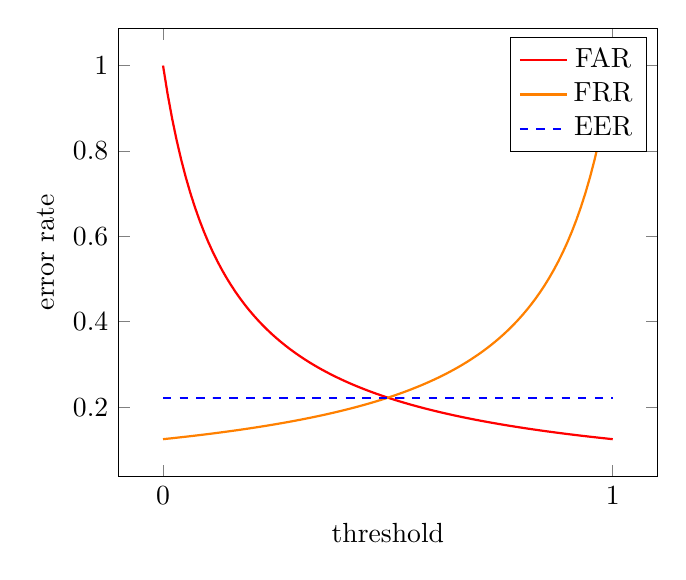
\begin{tikzpicture}
        \begin{axis}[
                xlabel=threshold,
                ylabel=error rate,
                xtick={1,8},
                xticklabels={0,1}
            ]
            \addplot[
                domain=1:8,
                samples=100,
                thick,
                color=red]{1/x};
            \addlegendentry{FAR};
    
            \addplot[
                domain=1:8,
                samples=100,
                thick,
                color=orange]{1/(9-x)};
            \addlegendentry{FRR};
    
            \addplot[
                domain=1:8,
                samples=100,
                dashed,
                thick,
                color=blue]{2/9};
            \addlegendentry{EER};
        \end{axis}
    \end{tikzpicture}
    \caption{\textit{False Acceptance Rate} and \textit{False Rejection Rate}
    for biometric authentication}
    \label{fig:eer}
\end{figure}

\section{Password Security}
Passwords which are short or badly chosen can easily be cracked. Brute-force or
dictionary attacks guess the password either randomly of from a list of known
(pass-)words. Brute-force attacks are easily feasible for passwords up to
\textasciitilde 8 characters in length, useful rules on possible guesses and
dictionary attacks can lead to success for even longer passwords. An advantage
for the attacker is when the attack can be executed \textit{offline}, such as by
stealing the file containing the password hashes. This removes the bottleneck of
the authentication mechanism of the target and allows for distributed attacks.

A common protection measure is to use a \emph{SALT}. A salt is a random value
that gets appended to the password before hashing, and then gets stored
alongside the password hash. While this does not protect a single password
against the mentioned attacks, it prevents reuse of a hash that has already been
calculated. Otherwise, it would be possible to just compare the hashes to known
hashes of popular passwords.

Another consideration is access to the password hashes. While the actual
cryptographic security is only influenced by the hash function, preventing
offline attacks by properly protecting the hashes forces the attacker to execute
much slower online attacks. Those online attacks can be slowed even further by
limiting the number of invalid authentication attempts or introducing an
increasing delay after failed authentication attempts (\textit{back off}), and
by using ``slow'' hash functions. The previously popular measure of password
aging (requiring passwords to be changed after a certain amount of time) is
discouraged, since it promotes the use of weak but easy to remember passwords.

Other attacks focus on the specific implementation of the authentication
mechanism and exploit vulnerabilities that allow login even without actually
obtaining the correct password, or allow changing or resetting passwords even
with insufficient privileges.

\subsection{Time Memory Trade-off}
In attacks on passwords a trade-off between time and memory has to be made, the
two extremes being the brute-force attack and the fully pre-calculated
dictionary/codebook attack.

One possible solution is a \emph{Variable Length Lookup Table}. Those rely on
hash chains: For many initial values, a chain of hashes (length $n_\text{max}$)
each is calculated. Only the initial and end-value are for each chain is then
stored. When a certain hash shall then be cracked, it will be hashed
$n_\text{max}$ times until a chain is found which end-state matches the
calculated hash. Once the chain is found, it can be restored using the stored
initial state which results in a chain containing the to-be-cracked hash and the
password as the state immediately preceding that value.

An improvement to lookup time can be made by making the chains variable length,
and introducing an end criterion, for example a certain number of zero-bits at
the end of the hash (\emph{Distinguished Codepoints}). This reduces the number
of end-lookups significantly.

Duplication arising from hash collisions are addressed by \emph{Rainbow Tables}:
A round-specific reduction function (hash space \textrightarrow password space)
is introduced. So even if a state is already present in a different chain (but
at another round in the chain), the original chain continues separately.

\section{Network Authentication}
The challenge of network authentication is that the communication has to be
established over an insecure channel. Passwords shall not be transmitted as
plaintext, but in encrypted form. Thus the problem quickly changes from
authentication to a key-distribution problem.

\subsection{Kerberos}
Kerberos is a network authentication protocol using symmetric cryptography. It
is best explained using an example:

Each organization has one authentication server, also called key distribution
center, and a ticket granting server TGS. The TGS hands out the authorization to
clients to use a certain service. This is done using tickets. A ticket for a
client to access a service includes a specific session key, the identity of the
client and a validity period. The ticket is encrypted using a key that only the
TGS and the service know. The client can not decrypt the ticket.

If a client $A$ wants to access a service $B$, $A$ first contacts the
authentication server. The server then provides $A$ with a session key between
$A$ and the TGS (encrypted using $A$s password), and a ticket for the TGS which
can provide TGS with the session key to talk to $A$.

The TGS can now provide $A$ with a session key between $A$ and $B$, and a ticket
for $B$ that provides $B$ with the session key.

Now $A$ and $B$ have a shared session key, and they can communicate.

Criticism of kerberos include the centrally controlled servers, and reliance on
synchronized clocks for timestamps. Session keys are known to the servers, not
only to the client and service. Also, the first message is not authenticated,
opening multiple attack vectors.

\subsection{Station to Station}
It has already been established that Diffie-Hellman is susceptible to
man-in-the-middle attacks (\cref{sec:diffiehellman}). A solution is to
authenticate the public keys $A$ and $B$ using digital signatures.

The station to station protocol now requires verification of signatures after
exchanging the public values $A$ and $B$: Bob signs both $A$ and $B$ with his
private signing key, Alice signs both $A$ and $B$ using her private signing key.
The signatures are encrypted using the shared secret key. Verification of the
signature now assures each party that no man in the middle who is exchanging the
keys is present.

This assumes however that the public signature verification keys are already
known.

\subsection{Perfect Forward Secrecy}
Perfect forward secrecy is given when the compromise of a long term secret such
as secret keys does not compromise the security of short term secrets used in
the past.

\subsection{Certificates}
A digital certificate links some public key to a person. The certificates
generally includes the public key, some identifier and a validity period. All
this is signed by the signature generation key of a trusted third party
(certification authority CA). This certificate can then be verified if the
verification key of the CA is known.

The \emph{certification authorities} play an important role in the \emph{public
key infrastructure}. Usually a number of CAs exist, which all operate under some
root CA. The root CA signs the public keys of the other CAs and such verifies
the validity of the CA. Those CAs can then sign public keys of users, after
verifying their identity.

The public key of the root CA has to be transmitted using a secure channel. This
is usually done by distribution via operating systems and browsers.

\subsubsection{X.509 Certificates}
X.509 is a standard for digital certificates. It specifies that the identifier
is in the hierarchical \textit{distinguished name (DN)} naming format. It also
specifies the fields in the certificate:
\begin{itemize}
    \item Version
    \item Serial number
    \item Signature algorithm
    \item Issuers DN
    \item Validity interval
    \item Subjects DN
    \item Subjects public key
    \item Issuers unique identifier
    \item Subjects unique identifier
    \item Extensions
    \item Signature
\end{itemize}
Extensions can for example control the key usage (signing emails, TLS web
server, etc).

PKIs have several problems, which become evident if a CA gets compromised. This
allows the attacker to for example issue certificates for any domain. The number
of CAs commonly in use is large, and many use weak security.

\subsection{PGP}
Pretty Good Privacy PGP provides an alternative approach to trust in a
decentralized fashion. It relies on the concept of users singing each others
keys. Each user has a keyring of public keys and signatures on them. If a user
receives a public key which is signed by many users they trust, they might also
trust the new public key.

There are different notions of trust: \emph{Owner trust} is the value of trust
someone assigns to a key in the keyring. Completely trusting a key implies also
trusting the other keys signed by this key.

\emph{Calculated trust} answers the question of whether to trust a public key
that was used. A chain of signatures is required, starting with some public key
in the keyring and ending with the key in question.

\emph{Key legitimacy} is calculated as
\begin{equation}
    L = \frac{x}{X}+\frac{y}{Y}
\end{equation}
with $x$ being the number of signatures with ``marginal'' trust, $y$ the number
of signatures with ``complete'' trust and $X$ and $Y$ the required corresponding
number of signatures.

\chapter{Access Control}
\label{chapter:access_control}
Access control combines authentication and authorization.
\Cref{chapter:authentication} showed how the identity of a subject can be
confirmed, the question is now whether the subject is \emph{authorized} to
access a specific resource. This decision is generally performed by a
\emph{reference monitor}, on the basis of some \emph{access policy}, which may
be set by an administrator or the owner of the object.To differentiate the terms
\textit{subject} and \textit{object}:

A \emph{subject} is the \textit{acting entity}, which intends to carry out an
operation requiring access. Examples include persons, processes or network
nodes. A subject can also be the object of an access operation at another time.

An \emph{object} is the unit that is \textit{being accessed}. Examples include
files and directories, database records, computers, processes, mailboxes or
applications.

The \emph{access operation} is the type of operation of a subject in relation to
an object. Different sets of access operations can be defined. A file system
might for example define \textit{read} and \textit{write} operations (or
\textit{observe} and \textit{alter}). There might be additional operation like
\textit{execute} or \textit{append}, which can be handled independently.

\section{Access Control Matrix}
The access policy can be described using an \textit{access control matrix}. The
matrix contains the set of every allowed operation for every possible pair of
subject and object. This however immediately presents a problem, as this
approach scales badly. For $N$ subjects (users) and $M$ objects (files), a $N
\times M$ matrix would have to be stored.

Two implementations of the access control matrix may be more appropriate
depending on the application:

\subsection{Access Control List}
In an Access Control List (\textit{ACL}), a list of subject-operation pairs is
stored with each object. A file might for example contain a list of all users
that have access to that file, and which exact operations they are allowed to
execute on the file. If a user is not allowed to interact with the file in any
way, the entry may be omitted.

\subsection{Capabilities}
In direct contrast to the ACL, in a capabilities based system the subjects
contain a list of objects and the corresponding operations which the subject is
authorized to execute on the object. In the file system example, each user would
contain a list of files which the user is allowed to access.

\section{Models for Access Control}
More detailed access control models are in use:
\begin{itemize}
    \item[DAC] \emph{Discretionary Access Control} is the approach as explained
          above. Access control decisions are based on a subject and object.
          Subjects define the access rights of an object (file owner for
          example).
    \item[MAC] \emph{Mandatory Access Control} is oriented towards clearance
          levels, as one might expect in a government or military setting. The
          access rights are usually defined system-wide, and are not changed by
          a subject. More information on this in \cref{sec:belllapadula}.
    \item[RBAC] In \emph{Role Based Access Control} access to objects is not
          defined per subject, but per \textit{role}. Roles are given to
          subjects, and may change.
    \item[ABAC] \emph{Attribute Based Access Control} is even more abstract,
          where both subjects and objects have attributes, and access control
          decisions are made by flexible comparison of attributes.
\end{itemize}

Real world systems often implement aspects of multiple of those models, and no
model is the best or definitive answer to access control.

\section{Example: Linux}
\todo[inline]{Linux access control, ACLs}

\section{Multilevel Security, Bell-Lapadula-Model}
\label{sec:belllapadula}
In multilevel security, both objects and subjects are classified. Classes may
for example be \textit{Unclassified}, \textit{Confidential}, \textit{Secret} and
\textit{Top Secret}. Access is only granted if the subject has at least the same
classification as the object. Access is denied if the subject has a lower
classification than the object. The \emph{Bell-Lapadula-Model} is an
implementation of this access control model:

To define this model, consider a set of subjects $S$, a set of objects $O$ and
the set of operations $A = \{\text{execute}, \text{read}, \text{append},
\text{write}\}$. For two security levels $a, b \in SL$, there always exists a
greatest lower bound $l \in SL: (l \leq a, l \leq b \text{ and } l
\text{minimal})$ and a least upper bound $h$.

The system is in a state at all times. A state is a triple $(b, M, f)$ with
\begin{itemize}
    \item $b \subseteq S \times O \times A$ the set of current accesses
    \item $M = (M_{so})_{s\in S, o\in O}$ the current access matrix
    \item $f = (f_s, f_c, f_o)$ with
          \begin{itemize}
              \item $f_s: S \mapsto SL$ the maximum clearance of each subject
              \item $f_c: S \mapsto SL$ the current clearance of each subject
                    (this requires $f_c(s) \leq f_s(s)$ for each subject $s$)
              \item $f_o: O \mapsto SL$ the security classification of each
                    object
          \end{itemize}
\end{itemize}

The current clearance $f_c$ is chosen by each subject, within the limit set by
the maximum clearance $f_s$.

A state is secure, if the following properties are met:
\begin{itemize}
    \item \emph{Simple Security Property}: For all $(s, o, a) \in b$ with
          $a=\text{read}$ or $a=\text{write}$: $f_o(o) \leq f_s(s)$ (Each
          subject which is currently reading or writing has the necessary
          maximum clearance)
    \item \emph{*-Property}:
          \begin{itemize}
              \item For all $(s,o,a)\in b$ with $a=\text{append}$: $f_c(s) \leq
                        f_o(o)$ \\ (No append operation is executed with higher
                        clearance than the object)
              \item For all $(s,o,a)\in b$ with $a=\text{write}$: $f_c(s) =
                        f_o(o)$ \\ (Each write operation is executed with
                        minimal clearance)
              \item For all $(s,o,a)\in b$ with $a=\text{read}$: $f_c(s) \geq
                        f_o(o)$ \\ (Each read operation is executed with a
                        sufficient current clearance)
          \end{itemize}
          This property enforces the correct selection of the current clearance
          $f_c$. Appending happens ``upwards'', writing on the same level, and
          reading ``downwards''.
    \item \emph{Discretionary Security Property}: For all $(s,o,a) \in b$: $a
              \in M_{s,o}$
\end{itemize}

\section{Multicategory Security}
\todo[inline]{multi category security}

\section{POSIX Capabilities}
POSIX capabilities are an implementation of a capability based access control
scheme. An example would be the right to open raw sockets on linux, which is
usually reserved to the root user. This is however necessary for the
\texttt{ping} utility, which should be accessible to every user, even without
setting the \texttt{setuid} bit on the binary. The POSIX capability system now
allows giving the specific right to open raw sockets to the specific binary.
This also adheres to the principle of least privilege a lot better than always
executing \texttt{ping} with full root rights. Capabilities are also not
reserved to files, but can be given to individual processes as well.

\input{chapters/05_malware.tex}
\chapter{OS Security}
\textit{Operating system-} and \emph{host-security} has the goals of protecting
stored data, running processes and the operating system itself. This
necessitates some form of authentication, to distinguish between users on a
multi-user system, as well as an access control system which assigns permissions
to users. A useful concept applied here is isolation, which is applied to users
and processes. Raw hardware access is usually restricted, and only allowed to
privileged code within the operating system. Protection against external access
may also be part of host security.

A core problem of host security is the \emph{confinement problem}: The problem
of preventing a server from leaking information that the user of the service
considers confidential.

\section{Concepts and Reference Monitors}
A \emph{reference monitor} is an abstract machine which mediates all accesses to
objects by subjects (see \cref{chapter:access_control}). Reference monitors can
be implement on any level of the system. Reference monitors in the systems
hardware include the MMU and privileged execution modes. Kernel level reference
monitors are for example implemented in the file system or capability system.
Applications can also contain reference monitors, which may be the case in web
server applications, or run completely inside another program which implements a
reference monitor such as the Java virtual machine or a database engine.

The \emph{security kernel} is the hardware, firmware and software of a trusted
computing base which implements the reference monitor. It must mediate all
accesses, be protected from modification and be verifiable as correct.

The \emph{trusted computing base (TCB)} is the totality of protection mechanisms
within a computer system. This includes hardware, firmware and software which is
responsible for enforcing a security policy. The enforcement of the security
policy must only depend on the TCB, the rest of the operating system need not to
be trusted.

\section{Virtualization and Mandatory Access Control}
\subsection{Virtualization}
There exist many reasons to use virtualization, but the goal of virtualization
from a security perspective is full isolation of systems and applications. The
possibility to roll back an entire system to a known-good state in case of
compromise also presents an advantage.

Levels of virtualization are distinguished based on the role and position of the
\emph{virtual machine monitor VMM}. In \emph{native virtualization}, the VMM
directly interfaces with the hardware. In \emph{user mode virtualization}, the
VMM only interfaces with the host OS, and not directly with the hardware. A
hybrid approach is \emph{dual-mode virtualization}, where a host OS exists, but
some form of direct access to the hardware by the VMM is possible.

The interaction of the VMM with the \emph{guest OS} provides another way of
categorization: In \emph{full virtualization}, the guest OS runs unmodified, as
on real hardware. This is usually assisted by various hardware extensions such
as \textit{AMD-V} and \textit{Intel VT-x}, special support by the MMU and
passthrough of system busses such as PCI.

\emph{Paravirtualization} refers to a mode of virtualization in which the guest
OS is aware of the virtualization and has some adaptations to the host OS.
Hardware drivers for example can be replaced with components that directly
interface with the VMM.

\subsection{Isolation}
Isolation is the main benefit of virtualization from a security perspective.
Errors in applications can be contained effectively, programs with different
security requirements can be separated, and malware analysis is possible without
effecting the host system. The host system can employ detailed monitoring, and
perform effective intrusion detection from the outside. The isolation of common
dependencies between applications prevents the compromise of multiple
applications by compromise of the common dependency.

As an example, a payment processor may be located in a dedicated VM with a
secure operating system. The non-critical application such as a frontend which
exposes a large attack surface runs in a separate VM and interfaces with the
payment application only through a closely monitored interface.

\subsection{Security Enhanced Linux}
Linux provides the \emph{Linux Security Module (LSM)} interface. Once a user
triggers a security sensitive activity in the kernel through a syscall (for
example: \texttt{read}), the LSM hook is executed, which the LSM module
registers. The LSM module can then for example deny the filesystem access.
\emph{SELinux} is such a module. SELinux supports a variety of mandatory access
control schemes, the main one discussed here is \emph{type enforcement}. The
idea is that both subjects and objects are assigned security labels. A central
security policy determines which subjects can execute which operations on the
objects based on the labels. The acting entity is always a process. Processes
are assigned to \emph{domains}, for which access rules to objects are specified.
SELinux supports two modes of handling processes without a specified domain:
assigning all of those to a default \texttt{unconfined} domain or creating an
individual domain for each process.

Files are tagged with security \emph{labels}. The label my include a user identity,
role, type or domain. The last field implements the type enforcement: for
regular files, this expresses the type of the object, but for executables this
determines the domain of the process once it is executed.

Beyond the simple type enforcement, \emph{roles} can be defined. Users can have
roles, and users can change the current role if they have sufficient privilege.
Specific rights can then be given to specific roles.

Multi-category and multi-level security is also implemented in SELinux,
implementing the Bell-Lapadula model (see \cref{sec:belllapadula}).

\subsection{AppArmor}
\todo[inline]{AppArmor: describe example from video 6b}

\section{Use-Case: iOS Security}
\todo[inline]{iOS Security}

\chapter{Embedded and Hardware Security}

Security in embedded systems is of special concern. Embedded systems are often
harder to patch, and often have direct real-world impact, sometimes in a safety
critical way. Non-mainstream operating systems are in use, and the CPU might not
offer all desired security features (see below). This results in a large attack
surface on a system that is not as well understood security-wise as desktop- or
server applications.

In the following, security will be considered from a lower level than before,
down to the hardware. Many of the security measures considered before can be
circumvented if lower-level access is present. Access control on a file system
for example is worthless if the attacker can connect the disk to another system
and dump all the contents. Software security is difficult if it relies on
libraries that can be exchanged by an attacker.

Placing security mechanisms at the lowest possible layer circumvents those
attacks.

\section{Introduction and x86 Privilege Levels}
At any point while an x86 processor is executing instructions, it is in some
\emph{privilege level} or \emph{protection ring}, usually indicated by a number
where higher numbers represent less privileged execution:

\begin{itemize}
    \item[(-1)] Virtual Machine Monitor, Hypervisor
    \item[0] Operating system kernel
    \item[1] Rest of the operating system
    \item[2] I/O Drivers etc.
    \item[3] Application software
\end{itemize}

Switching to a lower privilege level must be protected, while switching to a
higher level (less privileges) is usually easy. One important feature made
possible by this is protection of memory segments. Each memory segment contains
a Descriptor Privilege Level \textit{DPL}, and each process is assigned a
privilege level. If the Current Privilege Level \textit{CPL} > \textit{DPL}, the
CPU generates a protection fault and prevents access to memory accessible only
to lower privilege levels. This for example prohibits applications from
modifying operating system data structures.

Upgrading of the privilege level (setting it to a lower value) may happen for
example when a syscall is initiated and execution is passed to the operating
system. This provides a well defined ``gate'' to those privilege levels.

In order to prevent an application to misuse the privilege level of the syscall,
by for example instructing it to copy data into the process that the application
would otherwise not have access to, an additional \textit{Requested Privilege
Level} may be introduced (\emph{confused deputy problem}).

\section{Isolation and HW-based Attacks}
The privilege levels introduced above provide a means of isolation between the
operating and user programs, often called \textit{userspace} and
\textit{kernelspace}. Isolation is often advantageous to security as it provides
a barrier with defined interfaces between components. A ubiquitous form of
isolation is that between multiple processes on a single computer. Address
space, access rights and file descriptors are completely separate for multiple
processes. Special security-critical functions such as handling of private keys
may even be delegated to a dedicated hardware security module.

Attacks which circumvent those measures and leak data through channels other
than the predefined interfaces are called \emph{side-channel attacks}: Such
side-channels may be for example power consumption or electromagnetic emission
of a device. Countless such side-channels have been found, with varying degree
of real-world usage. Most mitigations against such attacks have been broken by
even cleverer side-channel attacks. Recent examples of side-channel attacks
exploit interference between adjacent DRAM cells in main memory or cachelines
that don't get evicted after branch prediction has failed.

\section{HW-based Security Mechanisms}
\subsection{Trusted Platform Module}
IDK, seems like something the copyright-industry would come up with...

\subsection{Physical Unclonable Functions}
See Rührmair et. al.
\chapter{Software Security}
Development of secure software impacts all areas of software development. Before
implementation, analysis of requirements includes identifying threats, risk and
potential damages. The system design shall adhere to principles such as defense
in depth, reduced complexity and the principle of least privilege. Features such
as authorization and authentication as well as secure data  storage have to be
considered during the design phase, and are often much more difficult to add at
a later stage.

The implementation should make use of coding standards and best practices to
avoid common errors. The programming language, compiler, IDE or analysis tools
can help with those tasks.

Various forms of testing and verification are vital to ensure the software
performs as expected, which is absolutely necessary in order to even consider
the security of the system. A special case of testing, \textit{fuzzing}, is
explained in more detail in \cref{sec:fuzzing}.

\section{Software Development}
The goal during development of secure software is to prevent vulnerabilities in
the program. A vulnerability is a particularly severe security flaw. Flaws in
software can be categorized:
\begin{itemize}
    \item \emph{Errors} are mistakes a developer makes during design or
          implementation.
    \item \emph{Faults or Bugs} are errors in the code.
    \item A \emph{Failure} is a deviation of a program from the specified or
          intended behavior.
\end{itemize}

\paragraph{Functional testing} is used to look for failures, with the goal to
avoid faults and bugs which can cause the program to fail during normal
operation.

\paragraph{Security testing} searches for faults and bugs that lead to security
vulnerabilities. Those bugs often don't result in a failure during normal use,
but may be exploited by an attacker.

The most typical software flaws include improper handling of user input and
out-of-bounds memory accesses.

Some software is particularly critical. This includes all software that is
exposed to external entities, by interacting with the network or accepting input
from the user. Software that runs with high privileges is critical in so far
that a compromise could easily lead to compromise of the entire system.
Similarly, software in which a failure has critical consequences such as
software handling confident data or critical infrastructure needs to be
especially protected.

Multiple crucial design principles can be identified:
\begin{itemize}
    \item \emph{Segmentation} ensures that in case of inevitable eventual
          compromise, a breach is contained to a specified part of the system.
    \item The \emph{least privilege} principle states that each system shall
          have the least required amount of privileges, in order to defend
          against easy privilege escalation.
    \item \emph{Defense in depth} refers to the type of segmentation, in that a
          architecture consisting of multiple layers of abstraction is easier to
          protect.
    \item The \emph{low complexity} principle refers to the fact that the
          simpler a system is organized, the easier it is to find errors and
          spot design mistakes.
\end{itemize}

\section{Fuzzing}
\label{sec:fuzzing}
Fuzzing is a way of automated testing of software that accepts some kind of
input. It consists of brute-forcing different input values and combinations
until the program crashes or some fault is detected. This enables finding
edge-cases which are not handled in the program and might lead to a
vulnerability.
\chapter{Network Security}
\section{Information Gathering}
The first step in attacking a networked environment is always to gather
information on how the network is structured, and which connections, hosts and
segments exist. It is important to know which services exist, as they might
represent possible attack vectors. The next step is identifying vulnerabilities,
and exploiting them. This often includes searching for systems with known
vulnerabilities. What follows is often some measure to ensure permanent control,
such as the installation of a rootkit or backdoor. This process may then be
repeated to gain control to additional systems.

\subsection{DNS}
DNS exposes a lot of information about a network. Brute-forcing reverse DNS
lookups for a targets IP range reveals domains or hostnames, which often reveal
the purpose or service of a system.

\subsection{whois}
\texttt{whois} provides information about an IP range, specifically details
about the organization and administrator responsible. Privacy regulations make
it possible to vastly reduce the information visible nowadays.

\subsection{traceroute}
Network topology can be examined using \texttt{traceroute}. This tool uses ICMP
packets with increasing TTL to find the address of each intermediate router
between the source and a target address. Executing this from multiple hosts to
multiple targets enables mapping the complete network.

\subsection{SMTP}
\subsection{Sniffing}
Tools such as tcpdump or wireshark allow passive recording and decoding of
network traffic. This allows direct retrieval of information transmitted in
plaintext, and a lot of information even with encrypted communication through
metadata.

\subsection{Scanning}
Active scanning of hosts and networks is possible through tools like
\texttt{nmap}. The goal is usually to find out on which TCP or UDP ports there
are applications listening.

\paragraph{TCP connect scanning} simply tries to establish a TCP connection with
the target. The typical packet sequence in a successful case would be
\texttt{SYN}, \texttt{SYN/ACK}, \texttt{ACK}. If no application is listening,
the sequence would be \texttt{SYN}, \texttt{RST/ACK}. This scanning technique is
fast and easy to execute, even for non-superuser users. Disadvantages include
that this only works for TCP, and is easy to detect even on application level.

\paragraph{TCP \texttt{SYN} scanning} is an alternative where no complete TCP
session is ever created. If the port is open and the target responds with
\texttt{SYN/ACK}, the connection is immediately aborted with \texttt{RST}, not
completing the three-way-handshake. This never creates a connection that the
application receives, making it a lot more difficult to detect. This however
also only works for TCP, and additionally requires superuser privileges to
execute.

\section{Attacks}
The TCP/IP family of protocols was not designed with security as an objective.
Various different attacks are possible:

\subsection{Routing Attacks}
Attacks on routing protocols can facilitate redirection of traffic through the
attackers systems, or blackhole the traffic for a denial of service attack.
Routing protocols currently in place are not very security focused, OSPF for
example uses simple authentication using plaintext passwords and MD5 hashes,
BGP4 relies on manual filters for incoming information.

Inside a subnet, techniques such as ARP spoofing are possible, which allow
redirection of traffic to the attackers machine just by responding to ARP
queries for the corresponding IP address (or the gateway). DHCP replies can be
forged in a similar way.

\subsection{DNS Attacks}
DNS attacks are of special importance since basically all internet communication
relies on DNS during initialization of the connection. If the attacker controls
the DNS server, they can redirect traffic intended for a specific domain to a
malicious server. One method of attacking is \emph{DNS cache poisoning}:

DNS makes use of a hierarchical architecture, and various levels of caching to
ease load on the root and authoritative servers. The attacker targets such a
caching server by triggering it to refresh the cache, for example by querying a
targeted domain, and then immediately delivering a malicious response which then
gets stored in the cache. While refreshing a cache entry, the server sends a
request with a specific \texttt{query ID} to the upstream server. For a response
to be accepted, the \texttt{query ID} has to match, but it is not verified in
any other way if the reply indeed originates from an upstream server instead of
a malicious attacker.

The \texttt{query ID} is traditionally simply incremented each request, which
means the attacker could easily guess it by querying the server for a domain, to
which they own the authoritative name server, and assuming that the
\texttt{query ID} for the to-be-poisoned request will be a subsequent number.
The attacker will send multiple replies with different \texttt{query ID}s, with
a high probability that one of them matches. If the reply arrives at the cache
before the legitimate reply, the attack has succeeded.

The challenges to the attacker are so far:
\begin{itemize}
    \item The entry must not be in the cache already
    \item The correct \texttt{query ID} must be guessed
    \item The response must arrive before the legitimate response
\end{itemize}

The most straightforward fix is to implement cryptographically secure random
\texttt{query ID}s.

It is however still possible to take over an entire nameserver/zone: The goal
here is to corrupt the cache entry for the authoritative nameserver in the
caching nameserver. Requests to the victim nameserver can be made for any
non-existing subdomain the target nameserver is responsible for. In the forged
response, a \texttt{NS} record is present containing the domain of the
legitimate authoritative nameserver, but the accompanying \texttt{A} record
points to a server the attacker controls. The ability to use arbitrary
subdomains that will not be cached makes guessing the \texttt{query ID}
feasible, combined with the fact that it is only 16bit long.

Additional mitigations include using the port number of the request as an
additional identifier, but this does only increase the effort in guessing, it
does not solve the underlying problem. A long term solution is DNSSEC
(\cref{sec:dnssec}).


\subsection{Man in the Middle Attacks}
The objective of a man-in-the-middle attack is to infiltrate an existing or new
connection. Both endpoints think they communicate with each other, when they are
actually both communicating with the attacker. The attacker can then both record
and modify the traffic, and this can even work with encrypted connections. If
the attacker spoofs the IP of a target web server for example, the client
establishes a TLS connection, and the real web server receives an incoming TLS
connection, but both connections are separate and are terminated at the
attacker. A mitigation is exchanging certificates while the connection is
established. The certificate is signed (transitively) by a root CA, which has a
public key that is known to the client in advance, usually by distribution with
the operating system or browser. The user can then be warned if the server did
not send a certificate, or sent a certificate that is not signed by a known CA.

\subsection{Denial of Service Attacks}
A wide variety of DOS attacks exist at every level of a system. All those have
one goal in common: to deplete some resource of the system, making it
unavailable.

In network settings, DDOS, \textit{distributed} denial of service, is often
considered. Here, the attacker makes use of a large number of hosts, via a
botnet for example, to overwhelm the target with traffic from many sources. This
makes this type of attack possible even if every attacking system is a lot less
powerful than the target. Those attacks usually target the network connection or
server resources (CPU, memory, etc) of the victim.

Multiple types of network DOS attacks exist, but one example is \emph{SYN
    flooding}: The client sends a massive number of TCP \texttt{SYN} packets to
    the target, but never answers with \texttt{ACK}, establishing a connection.
    This results in the server saving a status for each half-established
    connection, which starves its resources.

Protection against SYN flooding is provided by \emph{SYN cookies}: It avoids
saving state when a \texttt{SYN} packet arrives. This is done by using the
sequence number in the TCP packet, which gets incremented whenever a packet is
sent. One does not however has to start at 1 or increment by 1. The server
inserts a value into the sequence number of the \texttt{SYN/ACK} which can be
used later to recognize that packet. This is generated using a hash function
that takes information like the current time, the host IP and port as well as a
server secret as input. The client is expected to increment this by 1 when
returning the ACK. When the server receives it, it can ``decrypt'' or
reconstruct the value to verify that the client has sent a \texttt{SYN} before.

General protection measures against DOS attacks include special hardware
appliances which monitor the traffic and protect against unusual amounts of
traffic, overprovisioning of servers and use of scalable cloud resources and
CDNs.

Difficult to protect against are \emph{low-and-slow} attacks, which try to slow
down a server by sending specially crafted packets which are known to trigger
slow or performance intensive operations on the target.

\section{Security Mechanisms}

In addition to the aforementioned protective measures against specific attacks,
this section goes into detail on DNSSEC, and the more general topics of
firewalls and intrusion detection.

\subsection{DNSSEC}
\label{sec:dnssec}
The basic idea of DNSSEC is that the authoritative servers sign the records
using asymmetric cryptography. The caching resolvers can then verify the
signatures. The required key-hierarchy lends itself to the hierarchical model
which is already in place with DNS. A server signs its records with a \emph{zone
signing key}, which is signed using the servers \emph{key signing key}. A hash
of the KSK is available at the parent zones nameserver, making it possible to
verify the identity of the server up to the root zone.

Solutions such as DoT and DoH introduce TLS and HTTPS as transports for DNS,
with the goal of privacy. It is however questionable how useful such measures
are, as they only delegate the problem to the operator of the DNS server.

\subsection{Firewalls}
Firewalls reduce the attack surface of a network by reducing its exposure to the
internet as a whole. A firewall is a network component which separates multiple
network segments from each other. Traffic between the networks is controlled
according to a security policy.

Firewalls often filter packets, which is done on multiple levels:
\begin{itemize}
    \item Virus-/Java-/ActiveX filter for email and HTTP: This provides a
          similar approach as local antivirus software may take, but at a
          centralized location. Those filters can however be easily
          circumvented, using encryption or even just unusual compression
          methods.
    \item Content filters, which scan for specific addresses or keywords
    \item Anti-Spoofing filters which remove packets with forged addresses (such
          as IP spoofing)
\end{itemize}

A firewall can however perform a lot of additional functions:
\begin{itemize}
    \item Logging
    \item Authentication
    \item Enforcement of data protection
    \item Network Address Translation
\end{itemize}

All those functions and requirements indicate that the firewall is closely
related and integrated with routers, gateways on multiple levels, logging
facilities and services providing authentication and security policies.

\subsubsection{Security policies}
An important decision in firewall configuration is the \emph{base policy}. It
specifies how traffic is handled, for which no more specific rule exists.

\emph{Default-Deny} specifies that access is usually prohibited unless it is
explicitly allowed. The list of allowed services is provided by the
administrator. This makes deployment of new services difficult, and may
frustrate users since a lot of services are not available.

The alternative is \emph{Default-Allow}, where access is usually permitted
unless explicitly prohibited. This has the disadvantage from a security
perspective that all potentially dangerous services have to be blocked, which is
usually not known in advance.

\subsubsection{Filtering}
Network level filtering can be done on layer 3 or layer 4: Layer 3 filtering
works on IP datagrams and is based on the source and destination addresses.
Layer 4 filtering can additionally take the port number and direction of
connection (in case of TCP) into account.

Application level filtering is sometimes referred to as \emph{deep packet
inspection}, and can make protocol specific decisions such as allowing only
certain HTTP methods or URLs, or block emails to a specific domain even when
being transmitted to a common mail server.

Packet filters are usually fully transparent and as such independent from the
user, and can be implemented highly performant. Disadvantages include poor
logging capabilities, difficult to set-up rules, and difficult to filter
protocols which may require stateful inspection, and usually no interpretation
of streamed data.

\subsubsection{Application Gateways / Proxies}
Gateways or proxy servers prohibit direct transfer of data via lower levels, but
require a proxy for each application protocol, which implements that protocol
and inspects the data, before forwarding it. This automatically realizes the
default-deny policy. It also makes it possible to authenticate the user, handle
user sessions and interpret data streams. The application specific nature
facilitates detailed logging and convenient to set-up filter rules. The gateway
is however not transparent to the user, requires a separate proxy for each
service or application and thus usually operates with lower performance.

\subsubsection{Firewall Architectures}
In addition to a simple packet filtering router, which may be implemented by a
dual homed host, firewall architectures often include a \emph{demilitarized zone
(DMZ)}. This is a special area within the firewall, which contains servers that
need to be accessible from the internet. An architecture with an application
gateway places the gateway in the DMZ. Incoming and outgoing traffic passes
through the screening router, which redirects it through the application
gateway. 

Multiple routers may be placed in the DMZ, usually an exterior router
between the internet and the DMZ, and an interior router between the DMZ and the
LAN. This makes the DMZ a \textit{screened subnet}. Separating the routers
provides multiple advantages, for example increased resistance towards DOS from
the internet (interior router not affected).

Multiple such levels of screening are possible, for example with dedicated zones
for servers requiring external access, and for servers that are only accessible
from the internal LAN, with an intermediate router in between.

\subsubsection{IP Tables}
\texttt{iptables} is a software packet filter in linux. It contains multiple set
of rules depending on the path a packet takes.

Ingress is always controlled by the rules for the \textit{prerouting} chain,
egressing packets pass through the \textit{postrouting} chain.

Packets destined for a local process, or originating process go through the
\textit{input} and \textit{output} chains, packets that pass through the system
are handled by the \textit{forward} chain.

For each chain, the behavior is configured using the tables \textit{filter},
\textit{nat} (Network Address Translation) and \textit{mangle} (modification of
packets). \textit{Nat} is not relevant for \textit{input} and \textit{forward},
\textit{filter} is not relevant for \textit{pre-} and \textit{postrouting}.

Each rule in a table contain a \textit{match} parameter specifying which packet
it applies to, and an action to be taken for matching packets. Matching rules
can have many criteria, including data quotas, rate limiting, and to tome extent
deep packet inspection.

\subsection{Intrusion Detection}

\input{chapters/10_web_security.tex}
\input{chapters/11_privacy.tex}
\end{document}